
%(BEGIN_QUESTION)
% Copyright 2011, Tony R. Kuphaldt, released under the Creative Commons Attribution License (v 1.0)
% This means you may do almost anything with this work of mine, so long as you give me proper credit

Suppose operators submitted a ``trouble-call'' to your instrument shop, claiming sump V-15 had an excessive liquid level inside of it (as indicated by LIR-134), and that the pump was not pumping that level down as it should:

$$\includegraphics[width=15.5cm]{i0005rx01.eps}$$

\vskip 10pt

Identify at least three possible faults, each one independently capable of accounting for the high sump level indication.  Also, identify any diagnostic tests you could perform on this system to pinpoint the nature and location of the fault.

\vskip 20pt \vbox{\hrule \hbox{\strut \vrule{} {\bf Suggestions for Socratic discussion} \vrule} \hrule}

\begin{itemize}
\item{} Suppose this trouble-call came to you during a very cold winter day, when the outside temperature was well below freezing.  How might this alter the list of potential faults?
\item{} Explain the purpose for having {\it check valves} on the discharge lines of the two submersible sump pumps.
\item{} Identify some of the different pressure-measurement accessory devices visible in this P\&ID.
\end{itemize}

\underbar{file i03513}
%(END_QUESTION)





%(BEGIN_ANSWER)


%(END_ANSWER)





%(BEGIN_NOTES)

Possible faults include (but are not limited to):

\begin{itemize}
\item{} Steam tracing turned off for pipe section (assuming freezing weather)
\item{} Clogged filter S-401
\item{} Shut block valve before or after filter S-401
\item{} Level controller LC-133 defective
\item{} Low-level switch LSL-133 failed
\item{} Nitrogen purge gas supply failed (not purging)
\item{} Circuit breaker to pump(s) tripped
\end{itemize}

Pressure gauge PI-417 could be used to tell whether or not one of pumps was running, by noting whether there was significant pressure on the common discharge line.

\vskip 20pt \vbox{\hrule \hbox{\strut \vrule{} {\bf Virtual Troubleshooting} \vrule} \hrule}

This question is a good candidate for a ``Virtual Troubleshooting'' exercise.  Presenting the diagram to students, you first imagine in your own mind a particular fault in the system.  Then, you present one or more symptoms of that fault (something noticeable by an operator or other user of the system).  Students then propose various diagnostic tests to perform on this system to identify the nature and location of the fault, as though they were technicians trying to troubleshoot the problem.  Your job is to tell them what the result(s) would be for each of the proposed diagnostic tests, documenting those results where all the students can see.

During and after the exercise, it is good to ask students follow-up questions such as:

\begin{itemize}
\item{} What does the result of the last diagnostic test tell you about the fault?
\item{} Suppose the results of the last diagnostic test were different.  What then would that result tell you about the fault?
\item{} Is the last diagnostic test the best one we could do?
\item{} What would be the ideal order of tests, to diagnose the problem in as few steps as possible?
\end{itemize}

%INDEX% Measurement, pressure: troubleshooting
%INDEX% Process: oily water sump (realistic P&ID shown)

%(END_NOTES)

